% Apresentacao
% ------------------------------------------------------------------------
% ------------------------------------------------------------------------

\title{Monografia TCC}

\documentclass[
	% -- opções da classe memoir --
	12pt,				% tamanho da fonte
	%openright,			% capítulos começam em pág ímpar (insere página vazia caso preciso)
	%twoside,			% para impressão em verso e anverso. Oposto a oneside
    oneside,
	a4paper,			% tamanho do papel. 
	% -- opções da classe abntex2 --
	chapter=TITLE,		% títulos de capítulos convertidos em letras maiúsculas
	%section=TITLE,		% títulos de seções convertidos em letras maiúsculas
	%subsection=TITLE,	% títulos de subseções convertidos em letras maiúsculas
	%subsubsection=TITLE,% títulos de subsubseções convertidos em letras maiúsculas
	% -- opções do pacote babel --    
	english,			% idioma adicional para hifenização
	% french,				% idioma adicional para hifenização
	% spanish,			% idioma adicional para hifenização
	brazil				% o último idioma é o principal do documento    
	]{abntex2}
    
    %\renewcommand{\ABNTEXpartfontsize}{\normalsize}
	%\renewcommand{\ABNTEXchapterfontsize}{ \large}
	%\renewcommand{\ABNTEXsectionfontsize}{\normalsize}
	%\renewcommand{\ABNTEXsubsectionfontsize}{\normalsize}

% ---
% Pacotes básicos 
% ---
\usepackage{lmodern}			% Usa a fonte Latin Modern			
\usepackage[T1]{fontenc}		% Selecao de codigos de fonte.
\usepackage[utf8]{inputenc}		% Codificacao do documento (conversão automática dos acentos)
\usepackage{lastpage}			% Usado pela Ficha catalográfica
\usepackage{indentfirst}		% Indenta o primeiro parágrafo de cada seção.
\usepackage{color}				% Controle das cores
\usepackage{graphicx}			% Inclusão de gráficos
\usepackage{microtype} 			% para melhorias de justificação
\usepackage{todonotes}
\reversemarginpar % Coloca as anotações do lado esquerdo
\setlength{\marginparwidth}{2.8cm}


\definecolor{algColor}{RGB}{255,206,206} % rgb(255, 206, 206)

% Pacotes para algoritmos/pseudo-código
\usepackage{listings}

\renewcommand{\lstlistingname}{Programa}

\lstset
{ %Formatting for code in appendix
    language=C,
    basicstyle=\footnotesize,
    numbers=left,
    stepnumber=1,
    frame = single,
    showstringspaces=false,
    tabsize=2,
    breaklines=true,
    xleftmargin=10pt,
    breakatwhitespace=false,
    extendedchars=true,
    literate={á}{{\'a}}1 
             {ã}{{\~a}}1
             {é}{{\'e}}1
             {í}{{\'i}}1
             {õ}{{\~o}}1
             {ç}{{\c{c}}}1,
}

\renewcommand{\lstlistlistingname}{Lista de códigos}

% Configura a ``Lista de Códigos'' conforme as regras da ABNT (para abnTeX2)
\begingroup\makeatletter
\let\newcounter\@gobble\let\setcounter\@gobbletwo
  \globaldefs\@ne \let\c@loldepth\@ne
  \newlistof{listings}{lol}{\lstlistlistingname}
  \newlistentry{lstlisting}{lol}{0}
\endgroup

\renewcommand{\cftlstlistingaftersnum}{\hfill--\hfill}

\let\oldlstlistoflistings\lstlistoflistings
\renewcommand{\lstlistoflistings}{%
   \begingroup%
   \let\oldnumberline\numberline%
   \renewcommand{\numberline}{\lstlistingname\space\oldnumberline}%
   \oldlstlistoflistings%
   \endgroup}
% ---
% Pacotes adicionais, usados apenas no âmbito do Modelo Canônico do abnteX2
% ---
\usepackage{lipsum}				% para geração de dummy text
% ---


% ---
% Pacotes de citações
% ---
%\usepackage[brazilian,hyperpageref]{backref}	 % Paginas com as citações na bibl
\usepackage[alf, abnt-etal-cite=2]{abntex2cite}	% Citações padrão ABNT

% --- 
% CONFIGURAÇÕES DE PACOTES
% --- 

\usepackage{abntex_ufrr_dcc}


% PACOTES DE ALGORITMO

\usepackage{algpseudocode,algorithm}
% Declaracoes em Português

\algrenewcommand\algorithmicend{\textbf{FIM}}
\algrenewcommand\algorithmicdo{\textbf{FAÇA}}
\algrenewcommand\algorithmicwhile{\textbf{ENQUANTO}}
\algrenewcommand\algorithmicfor{\textbf{PARA}}
\algrenewcommand\algorithmicforall{\textbf{PARA TODO}}
\algrenewcommand\algorithmicif{\textbf{SE}}
\algrenewcommand\algorithmicthen{\textbf{ENTÃO}}
\algrenewcommand\algorithmicelse{\textbf{SENÃO}}
\algrenewcommand\algorithmicreturn{\textbf{RETORNE}}
\algrenewcommand\algorithmicfunction{\textbf{FUNÇÃO}}
% New definitions
\algnewcommand\algorithmicswitch{\textbf{ESCOLHA}}
\algnewcommand\algorithmiccase{\textbf{CASO}}
\algnewcommand\algorithmicassert{\texttt{assert}}
\algnewcommand\Assert[1]{\State \algorithmicassert(#1)}%
% New "environments"
\algdef{SE}[SWITCH]{Switch}{EndSwitch}[1]{\algorithmicswitch\ #1\ \algorithmicdo}{\algorithmicend\ \algorithmicswitch}%
\algdef{SE}[CASE]{Case}{EndCase}[1]{\algorithmiccase\ #1}{\algorithmicend\ \algorithmiccase}%
\algtext*{EndSwitch}%
\algtext*{EndCase}%


% Rearranja os finais de cada estrutura
\algrenewtext{EndWhile}{\algorithmicend\ \algorithmicwhile}
\algrenewtext{EndFor}{\algorithmicend\ \algorithmicfor}
\algrenewtext{EndIf}{\algorithmicend\ \algorithmicif}
\algrenewtext{EndFunction}{\algorithmicend\ \algorithmicfunction}

% O comando For, a seguir, retorna 'para #1 -- #2 até #3 faça'
\algnewcommand\algorithmicto{\textbf{até}}
\algrenewtext{For}[3]%
{\algorithmicfor\ #1 $\gets$ #2 \algorithmicto\ #3 \algorithmicdo}


% ---
% Configurações do pacote backref
% Usado sem a opção hyperpageref de backref
%\renewcommand{\backrefpagesname}{Citado na(s) página(s):~}
% Texto padrão antes do número das páginas
%\renewcommand{\backref}{}
% Define os textos da citação
%\renewcommand*{\backrefalt}[4]{
%	\ifcase #1 %
%		Nenhuma citação no texto.%
%	\or
%		Citado na página #2.%
%	\else
%		Citado #1 vezes nas páginas #2.%
%	\fi}%
% ---

% ---
% Informações de dados para CAPA e FOLHA DE ROSTO
% ---
  \titulo{DETECÇÃO DE OBJETOS PARCIALMENTE OBSERVÁVEIS EM AMBIENTE AQUÁTICO COM ALTA TURBIDEZ }

\autor{PEDRO DANIEL DA SILVA GOHL}
\local{Boa Vista - RR}
\data{2017}
\orientador{DSc. Herbert Oliveira Rocha}

\tipotrabalho{Monografia}

\preambulo{Monografia de Graduação apresentada ao Departamento de Ciência da Computação da Universidade Federal de Roraima como requisito parcial para a obtenção do grau de Bacharel em Ciência da Computação.}

%Trabalho de conclusão de curso  na área de Verificação de Software desenvolvido na UFRR com o %objetivo \textcolor{red}{VERIFICAR O PADRÃO DOS OUTROS TCC} de gerar casos de teste para %sistemas embarcados críticos	

% ---

%-- Informações de dado para a FOLHA DE APROVAÇÃO
\renewcommand{\dataDefesa}{?}
\renewcommand{\orientadorBanca}{?}
\renewcommand{\primeiroMembroBanca}{?}
\renewcommand{\segundoMembroBanca}{?}

% ---
% Configurações de aparência do PDF final

% alterando o aspecto da cor azul
\definecolor{blue}{RGB}{41,5,195}

% informações do PDF
\makeatletter
\hypersetup{
     	%pagebackref=true,
		pdftitle={\@title}, 
		pdfauthor={\@author},
    	pdfsubject={\imprimirpreambulo},
	    pdfcreator={LaTeX with abnTeX2},
		pdfkeywords={abnt}{latex}{abntex}{abntex2}{trabalho acadêmico}, 
		colorlinks=true,       		% false: boxed links; true: colored links
    	linkcolor=black,          	% color of internal links
    	citecolor=black,        		% color of links to bibliography
    	filecolor=magenta,      	% color of file links
		urlcolor=black,
		bookmarksdepth=4
}
\makeatother
% --- 

% --- 
% Espaçamentos entre linhas e parágrafos 
% --- 

% O tamanho do parágrafo é dado por:
\setlength{\parindent}{1.3cm}

% Controle do espaçamento entre um parágrafo e outro:
\setlength{\parskip}{0.2cm}  % tente também \onelineskip

% ---
% compila o indice
% ---
\makeindex
% ---

% ----
% Início do documento
% ----
\begin{document}

% Retira espaço extra obsoleto entre as frases.
\frenchspacing 

% ----------------------------------------------------------
% ELEMENTOS PRÉ-TEXTUAIS
% ----------------------------------------------------------
% \pretextual

% ---
% Capa
% ---
\imprimircapa
% ---

% ---
% Folha de rosto
% (o * indica que haverá a ficha bibliográfica)
% ---
\imprimirfolhaderosto
% ---

% ---
% Inserir folha de aprovação
% ---
\imprimirfolhadeaprovacao
% ---
% Dedicatória
% ---
\begin{dedicatoria}
   \vspace*{\fill}
   \centering
   \noindent
   \textit{ } \vspace*{\fill}
   Dedico esse trabalho a minha mãe e a minha namorada, peças fundamentais do meu sucesso.
\end{dedicatoria}
% ---

% ---
% Agradecimentos
% ---
\begin{agradecimentos}
Agradecer minha força de vontade imensa de ter conseguido focar em algo até o fim.

\end{agradecimentos}
% ---

% ---
% Epígrafe
% ---
\begin{epigrafe}
    \vspace*{\fill}
	\begin{flushright}
		\textit{}
	\end{flushright}
\end{epigrafe}
% ---

% ---
% RESUMOS
% ---

% resumo em português
\setlength{\absparsep}{18pt} % ajusta o espaçamento dos parágrafos do resumo
\begin{resumo}


 \vspace{\onelineskip}
 
 \noindent 
 \textbf{Palavras-chaves}: 
\end{resumo}

\begin{resumo}[Abstract]
 \begin{otherlanguage*}{english}
   

   \vspace{\onelineskip}
 
   \noindent 
   \textbf{Key-words}: 
 \end{otherlanguage*}
\end{resumo}
% ---
% inserir lista de ilustrações
% ---
\pdfbookmark[0]{\listfigurename}{lof}
\listoffigures*
\cleardoublepage
% ---

% ---
% inserir lista de tabelas
% ---
\pdfbookmark[0]{\listtablename}{lot}
\listoftables*
\cleardoublepage
% ---

% ---
% inserir lista de abreviaturas e siglas
% ---
\begin{siglas}
  \item[e\&g] Verificação e validação de \textit{software}
  
\end{siglas}
% ---

% ---
% inserir lista de símbolos
% ---
% \begin{simbolos}  
%   \item[$ \Gamma $] \todo{Atualizar esta lista!} Letra grega Gama
%   \item[$ \Lambda $] Lambda
%   \item[$ \zeta $] Letra grega minúscula zeta
%   \item[$ \in $] Pertence
% \end{simbolos}
% % ---

% ---
% inserir o sumario
% ---
\pdfbookmark[0]{\contentsname}{toc}
\tableofcontents*
\cleardoublepage
% ---



% ----------------------------------------------------------
% ELEMENTOS TEXTUAIS
% ----------------------------------------------------------
\textual
% ----------------------------------------------------------
% Introdução
% ----------------------------------------------------------
\chapter{INTRODUÇÃO}
Com o aumento da complexidade dos sistemas computacionais, diversas
companhias e organizações estão
rotineiramente lidando com software que contêm milhares de linhas de
código, escritos por diferentes pessoas, e que usam diferentes
linguagens, ferramentas e estilos \cite{Hoder:2011}. Adicionalmente,
estes sistemas de software, devido ao curto espaço de tempo de
liberação do produto ao mercado, precisam ser desenvolvidos
rapidamente e atingir um alto nível de qualidade. Porém, os
programadores cometem enganos.
\par
Isso pode ser visto quando um programador se equívoca ao escrever
um requisito do sistema, como a alteração
de uma condição de $x \leq 10$ para $x < 10$, tempo e
esforço são gastos para encontrar e corrigir estes tipos de erro
\cite{Gupta:2009}. Como consequência destes fatores, os erros durante
o desenvolvimento de software se tornam mais comuns. Desta forma, faz-se
necessário que as aplicações sejam projetadas tomando em consideração os
requisitos de previsibilidade e confiabilidade, em
aplicações de sistemas críticos esses requisitos devem ser ainda mais
restritos, onde diversas restrições (como tempo
de resposta e precisão dos dados) devem ser atendidas e mensuradas de
acordo com os requisitos do usuário, caso contrário uma falha pode
conduzir a situações catastróficas \cite{Rocha:2015tese}. Por exemplo, o erro de cálculo da
dose de radiação no Instituto Nacional de Oncologia do Panamá que
resultou na morte de 23 pacientes \cite{Wong:2010, Merz:2012}.


\par
Inspecionar manualmente um \textit{software} é uma tarefa complexa, assim, é comum defeitos no software passarem despercebidos que podem interromper o seu funcionamento. 
%acabarem ocorrendo erros durante sua execução uma análise e com isso não gerar os casos de %teste necessários, o que acaba prejudicando a qualidade do sistema. 
Por exemplo, em sistemas embarcados com uso continuo que podem gerar vários estados possíveis de execução. Uma forma de evitar isso é a utilização de técnica de verificação formal automatizadas, através delas é possível verificar o sistema garantindo a qualidade do \textit{software}, pois através de métodos formais é possível gerar todos os casos de testes necessários para validação do sistema \cite{dsilva:2008}. Teste é um modo objetivo de verificar a corretude da implementação de um sistema, detectando algum comportamento inesperado em um caminho, testes não garantem que todo o programa está funcionando, apenas garantem que o programa está correto para determinado conjunto de testes. Métodos formais são considerados a forma rigorosa de verificar \textit{software} e analisar os sistemas com mais precisão, pois são capazes de gerar um conjunto de testes ideal para analisar o sistema \cite{ding:2008}.


\par
A verificação formal tem desempenhado um papel importante para
assegurar a confiabilidade e a qualidade no desenvolvimento de
aplicações críticas (como \textit{softwares} para piloto automático de aviões). 
Segundo \citeonline{Bensalem:1999}, \textit{model
checking} é uma técnica baseada em métodos formais utilizados para provar propriedades de programas. O \textit{model checking} é uma técnica automatizada que, dado um modelo de estados finitos de um sistema e uma propriedade formal, sistematicamente checa se a propriedade é verdadeira para o modelo \cite{Baier:2008}.Esta técnica gera uma busca exaustiva no espaço de estados do modelo para
determinar se uma dada propriedade é válida ou não \cite{Baier:2008}. A principal razão para o sucesso da técnica \textit{model checking} se dá por funcionar de maneira automática, não havendo necessidade da intervenção do usuário. Entretanto, a técnica \textit{model checking} ainda possui algumas dificuldades, tais como: lidar com a explosão do espaço de estados do modelo, integração com outros ambientes de testes e tratamento e análise de contra-exemplos \cite{Clark:2008}.

\par
Este trabalho visa aperfeiçoar o método Map2Check \cite{Rocha:2015}, que visa a geração automática de casos de testes para a verificação de gerenciamento de memória de programas escritos em C, sendo a geração desses testes baseadas em
assertivas extraídas de propriedades de seguranças geradas por ferramentas de
\textit{Bounded Model Checking}. No trabalho do Map2Check, \citeonline{Rocha:2015}
comentam sobre a dificuldade em se fazer a análise diretamente em códigos fontes escritos em C
e indica a utilização de uma representação intermediário do código do programa ou o uso de instrumentação em código binário nos seus trabalhos futuros, como uma solução para o problema, outro problema com o uso da linguagem C é percorrer o código com estruturas de alto nível, sendo complexo adicionar execução simbólica de forma automática. Neste sentido, as melhorias para o método Map2Check consiste em adicionar: 
%utilizar instrumentações em código intermediário com o LLVM:
1) a ferramenta Clang como \textit{front-end} para programas em C \cite{LLVM:2017}; 
2) o \textit{framework} LLVM como base para aplicações de transformações de código utilizando a representação intermediária LLVM \textit{bitcode} \cite{LLVM:2017}; e
3) o Klee para execução simbólica de código baseado em LLVM \cite{Cadar:2008:KUA}; 

\par
O \textit{Low-Level Virtual Machine} (LLVM) é um \textit{framework} de compilação cujo objetivo é fazer análises de programas e transformações que fiquem disponível para \textit{softwares} arbitrários de uma maneira que seja transparente ao programa original, por meio de: (a) o uso de uma representação intermediária (LLVM IR) de código capaz de descrever ações de análise e transformação de forma simples; e (b) uma infraestrutura de compilação capaz de tirar o maior proveito dessa linguagem \cite{Lattner:2004}. O \textit{framework} LLVM é utilizado por empresas como \textit{Apple Inc.}, \textit{Intel}, \textit{NVIDIA}, \textit{Sony Interactive Entertainment} \cite{LLVM:2009} e \textit{Google} \cite{LLVM:2011} por ser uma plataforma estável e robusta. \citeonline{Kim:2015} utiliza LLVM para fazer transformações de código (para otimizações) Android.

\par
O aprimoramento do Map2Check \cite{Rocha:2015} neste trabalho, tem como base métodos adotados em trabalhos como o LEAKPOINT \cite{Clause:2010} e o SYMBIOTIC 3 \cite{Chalupa:2016} 
que exploram o uso de técnicas de compiladores para analisar códigos-fonte 
em C para fazer a instrumentação dos mesmos. A diferença para as versões 
anteriores do Map2Check será na utilização de código intermediário usando LLVM IR, ou seja, a partir de um programa em C, será gerado um código LLVM IR, onde
faremos a instrumentação do mesmo e assim poderemos validar as
propriedades de segurança desejadas, como desalocações inválidas e vazamentos de memória. Utilizar uma linguagem intermediária tem a vantagem de que embora o foco do projeto seja a linguagem C, qualquer código em uma linguagem de programação que for compilada para LLVM IR, poderá ser
analisado pelo Map2Check.


% ----------------------------------------------------------
% MOTIVAÇÃO
% ----------------------------------------------------------
\section{Motivação}

A grande quantidade de áreas distintas para sistemas de \textit{software} de alto risco cria uma necessidade de um alto grau de confiabilidade. Uma falha em um sistema ambiental, militar, médico ou aerospacial pode criar um problema catastrófico. Sendo assim, um dos motivos deste trabalho é a necessidade de garantir a corretude de sistemas, que é acompanhada  pelo aumento da complexidades dos mesmo, ao mesmo tempo em que, por pressão econômica os prazos de entrega diminuem. O aumento da complexidade juntamente com a diminuição no prazo tornam mais difícil a tarefa de verificação do sistema a ser entrega. Isto motiva a pesquisa por formas automáticas de verificação e correção de \textit{software} \cite{dsilva:2008}

Um tipo de falha que pode impactar na performance e na corretude da aplicação é vazamentos de
memória. Em linguagens de programação como C, uma função de alocação reserva um espaço
previamente livre de memória (chamaremos de \texttt{m} esse espaço) e retornam um ponteiro 
(chamaremos de \textit{p} esse ponteiro) que aponta para o primeiro endereço dessa espaço
alocado. Normalmente, um programa armazena e somente então utiliza \textit{p}, ou algum outro
ponteiro derivado de \textit{p}, para interagir com \textit{m}. Quando \textit{m} não for mais
necessário, o programa deverá mandar \textit{p} para uma função de desalocação. Um vazamento
ocorre se, por algum erro durante o gerenciamento da memória, \textit{m} não é desalocado no
tempo correto \cite{Clause:2010}.

Os vazamentos por não gerarem um erro fatal (onde um sistema para sua execução) muitas vezes 
passam despercebidos (em 2009 mais de 100 vazamentos de memória foram reportados no navegador
Firefox), tipicamente esse vazamentos só são detectados após eles consumirem uma grande parte
da memória do sistema, causando assim impacto em todas as aplicações rodando no sistema. 
Por essas sérias consequência e ocorrências comuns, muitas técnicas foram criadas para os
detectar, porém em muitas situações não são técnicas simples de se aplicar \cite{Clause:2010}.



% ----------------------------------------------------------
% PROBLEMA
% ----------------------------------------------------------
\section{Definição do Problema}
A verificação de gerenciamento de memória é uma tarefa importante para evitar comportamentos inesperados de programas, por exemplo, uma violação na propriedade de segurança de um ponteiro resulta em um endereço errado, que pode acabar produzindo uma saída incorreta do programa e não necessariamente um erro. Um vazamento de memória não produz nenhum sintoma que seja visível facilmente ou detectado imediatamente como um erro ou a saída de um valor errado. Entretanto, vazamentos de memória geralmente continuam sem ser observados até consumirem uma grande porção da memória disponível no sistema, com isso, pode-se gerar em um impacto negativo em outras aplicações que estiverem sendo executadas no mesmo sistema \cite{Clause:2010}. Devido as sérias consequências e ocorrências comuns de erros de gerenciamento de memória, ainda existem campos de pesquisa aberto para aprimorar a detecção de error \cite{Rocha:2015tese}

%O \textit{model checking} contém várias vantagens em relação a outras técnicas \cite{Clark:2008}, algumas dessas vantagens seriam:
%\begin{itemize}
%\item O usuário de um \textit{model checker} não necessita construir provas de corretude
% \item O processo de verificação é automático
% \item \textit{Model checking} é rápido se comparado a outros métodos
% \item Se uma especificação não for satisfeita, o \textit{model checker} produzirá um contra-exemplo do caminho da execução, demonstrando o porque a especificação não está segura.
% \item Lógicas temporais podem ser facilmente expressas
% \end{itemize}
%
% Assim como \citeonline{Clark:2008} descreveu as vantagens ele também comenta algumas desvantagens do \textit{model checking}
% \begin{itemize}
% \item O \textit{model checking} não comprova o erro identificado no programa
% \item A escrita de especificações nem sempre é uma tarefa trivial
% \item O problema da explosão de estados, que é causado devido ao grande número dos estados de um sistema, podendo chegar a números exponenciais
% \end{itemize}
% Observando essas desvantagens, pode-se identificar campos de pesquisa em aberto, \citeonline{Clarke:2009} comenta sobre como a utilização de execução simbólica poderia simplificar o problema da explosão de estados

%TODO: Melhorar o problema
O problema considerado neste trabalho é expresso na seguinte questão:
\textbf{Como complementar e aprimorar a verificação de propriedades de
  segurança de memória, com foco em aritmética de ponteiros e vazamentos de memória, 
  com aplicação na linguagem de programação C?}

  
% ----------------------------------------------------------
% OBJETIVOS
% ----------------------------------------------------------
\section{Objetivos}
O objetivo principal deste trabalho é aprimorar um método para 
%aprimorar 
a verificação de propriedades de segurança de memória em 
software escritos na linguagem de programação C, por meio 
de transformações de código e uso da técnica \textit{ model checking}. 

Os objetivos específicos são:
\begin{enumerate}
\item Demonstrar melhorias em um método de geração e verificação 
  de casos de teste estruturais, baseado nas propriedades de 
  segurança de gerenciamento de memória.
  
\item Propor uma técnica para instrumentação de programas escrito em
  C, adotando técnicas de compiladores como análise de representações
  intermediaria de código.
    
\item Propor uma técnica baseada em execução simbólica para gerar
  dados de teste e identificação de localizações de erro em programas
  escritos em C.
   
\item Validar a aplicação dos métodos sobre \textit{benchmarks} públicos de
  programas em C, a fim de examinar a sua eficácia e aplicabilidade.
\end{enumerate}


% ----------------------------------------------------------
% METODOLOGIA
% ----------------------------------------------------------
\section{Metodologia Proposta}
Esta seção descreve as principais etapas que foram identificadas para alcançar os objetivos desta proposta de projeto. Estas etapas fornecem os passos necessários e direções para desenvolver o método proposto e podem ser descritas em três diferentes fases como segue: 
análise do domínio, metodologia proposta e validação da metodologia.
%
Na etapa de análise de domínio, toda a teoria necessária para entender os métodos, técnicas e ferramentas aplicadas à verificação e teste de software são analisadas e avaliadas. 
%
Na fase da metodologia proposta, uma versão inicial da metodologia para o desenvolvimento do 
método proposto, tem como foco uma ou mais restrições, e seu escopo serão precisamente definidos e propostos. 
%
Depois disso, esta metodologia é mais adiante refinada na fase de validação aplicando-a na verificação dos estudos de caso, visando uma avaliação experimental da solução proposta.


\par
Com o intuito de realizar as atividades deste trabalho, uma abordagem iterativa e incremental é 
usada com o propósito de reduzir riscos e incertezas. Sendo assim, para cada incremento do
projeto do trabalho, as três etapas nomeadas neste trabalho como análise do domínio, metodologia proposta e validação da metodologia podem ser tratadas com diferentes ênfases em cada fase do trabalho.
\par
Por exemplo, no início do trabalho, a análise de domínio provavelmente terá maior ênfase do que as outras fases metodologia proposta e validação da metodologia. Na metade do trabalho, a fase de metodologia proposta provavelmente terá mais ênfase do que as outras duas fases. Finalmente, a fase de validação da metodologia provavelmente terá mais ênfase no fim do projeto de pesquisa. A principal razão para adotar uma abordagem iterativa e incremental é desenvolver o projeto incrementalmente, permitindo assim tirar vantagem do que foi aprendido durante cada incremento do projeto \cite{Schwaber:2002}.

% ----------------------------------------------------------
% CONTRIBUIÇÕES
% ----------------------------------------------------------
\section{Contribuições Propostas}
As contribuições proposta por esse trabalho são: 
\begin{enumerate}
\item A implementação e avaliação de um método para a verificação e teste de programas em C. 
      O método proposto gera automaticamente casos de teste baseada em propriedades de segurança geradas através da instrumentação de código. Essas propriedades estão relacionadas à gerenciamento de memória e alcançabilidade de estados no programa.
      
\item  Este trabalho apresenta para o método proposto, o desenvolvimento e implementação de um 
      rastreador de endereços de memória baseado em representação intermediária (LLVM-IR) para auxiliar na verificação das propriedades do programa. Assim, esta contribuição auxilia na integração de técnicas formais de forma automática. 
      
\item Este trabalho visa contribuir com método Map2Check \cite{Rocha:2015}, consiste em 
     adicionar: 
     1) a ferramenta Clang como \textit{front-end} para programas em C \cite{LLVM:2017};
     2) o \textit{framework} LLVM como base para aplicações de transformações de código utilizando a representação intermediária LLVM \textit{bitcode} \cite{LLVM:2017}; e
     3) o Klee para execução simbólica de código baseado em LLVM \cite{Cadar:2008:KUA}.
\end{enumerate}
     
\section{Organização do Trabalho}
A introdução deste trabalho apresentou: o contexto, definição do problema, motivação, objetivos, metodologia e contribuições dessa pesquisa. Os capítulos restantes são organizados da seguinte forma:
\par
No \autoref{chapter:conceitos} \textbf{Conceitos e Definições}, são apresentados os conceitos abordados neste trabalho, especificamente: Verificação e Validação de \textit{Software}, Propriedades de Segurança, \textit{Bounded Model Checking}, Execução Simbólica e Técnicas de Compiladores.
\par
No \autoref{chapter:correlatos} \textbf{Trabalhos Correlatos}, são analisados os trabalhos correlatos ao método Map2Check.
%, como a versão anterior, o SYMBIOTIC 3 e o LEAKPOINT.
\par
No \autoref{chapter:metodo} \textbf{Método Proposto}, é descrito as etapas de execução do novo método proposto ao Map2Check.
% de forma que o leitor possa reproduzir a técnica. 
Em especial, são descritos: Geração da representação intermediária; Biblioteca para rastreamento de endereços de memória e assertivas; Instrumentação de funções; e Verificação do  do programa analisado. Por fim é apresentado o cronograma das atividades deste trabalho.
\par
No \autoref{chapter:resultados} \textbf{Resultados Experimentais}, descreve-se a execução de uma avaliação experimental sobre o método proposto, bem como, 
%descrevendo o \textit{benchmark} da SV-COMP utilizado e no fim é feita 
uma análise dos resultados obtidos, onde comparamos o novo Map2Check com outras ferramentas. 
\par
E por fim no \autoref{chapter:consideracoes} \textbf{Considerações parciais e trabalhos futuros}, apresenta-se as considerações parciais e os trabalhos futuros a serem desenvolvidos. 


% ----------------------------------------------------------
% Conceitos e Definições
% ----------------------------------------------------------
\chapter{Fundamentação teórica}
\label{chap:fund_teo}
	Este capítulo tem como objetivo apresentar a fundamentação teórica para o entendimento deste trabalho, no qual serão abordados conceitos de: Sistemas Embarcados, Modelos Formais para verificação de sistemas, Visão Computacional e Reconhecimento de Padrões.
  
    
\section{Sistemas Embarcados} 
Sistemas embarcados são sistemas baseados em microprocessadores ou microcontroladores, construídos para executar uma função ou grupos de funções programadas. Não são projetados para serem reprogramados da mesma forma que computadores pessoais \cite{heath:2002}.
%De acordo com \citeonline{heath:2002}, um sistema embarcado é um sistema baseado em um microprocessador ou microcontrolador, construído para executar uma função ou um grupo de funções programadas. Sistemas embarcados não são projetados para serem reprogramados como computadores pessoais são.
Um dos exemplos citados por \cite{heath:2002} como sistema embarcado é uma máquina de lavar, que possui vários ciclos de lavagem, painéis para acompanhar os ciclos e controle dos motores e bombas de água.
    
Já \citeonline{vahid:2002} definem sistemas embarcados como qualquer sistema que não seja um computador pessoal com as seguintes características:\begin{itemize}
\item Função única: Sistemas que são programados para um tarefa específica, que pode se repetir várias vezes.
\item Fortemente limitado: Sistema com limitações definidas nas suas métricas de projeto, como de desempenho, consumo de energia, preço e dimensões.
\end{itemize}

De acordo com \citeonline{schlett:1998}  um sistema embarcado baseado precisa executar uma tarefa específica com o menor custo energético e monetário possível. O custo energético é um dos grandes desafios encontrados no desenvolvimento de sistemas embarcados.
 

\subsection{Microcontroladores x Microprocessadores}
 Computadores modernos são baseados em microprocessadores, permitindo-os realizar várias funções, enquanto outros sistemas baseados em microcontroladores são limitados a apenas um ciclo repetido da mesma tarefa.\cite{heath:2002}
%Segundo \citeonline{white:2011} define microcontroladores como processadores com componentes atrelados a ele, com memória re-programável

Sistemas embarcados derivaram de processadores desenvolvidos para o mercado de computadores domésticos, com algumas diferenças no consumo energético, preço e componentes atrelados à \textit{CPU}. Outras diferenças são o tempo de resposta de interrupções, a quantidade de memória e portas paralelas.
\cite{schlett:1998}


\subsection{Internet das Coisas(IoT)}

A internet das coisas irá interligar todos os dispositivos atraves de sistemas embarcados, formando uma rede de dados, inteligente, ubíqua e distribuída. Os dispositivos podem trazer avanços que irão melhorar a qualidade de vida, facilitando a comunicação entre pessoas e dispositivos \cite{xia:2012}.
%\citeonline{xia:2012} afirma que a Internet das coisas irá interligar todos os dispositivos atraves de sistemas embarcados interligados por uma rede inteligente e ubíqua. 

Todos os dispositivos ao nosso redor estarão conectados a internet, isso irá resultar numa enorme quantidade de dados que terão de ser processados e apresentados sem falhas de forma eficiente. A computação em nuvem pode oferecer uma infraestrutura  de ponta a ponta, entre o dispositivo e o servidor satisfazendo essa demanda de qualquer lugar.\cite{Gubbi:2013} 

\subsection{Baixo consumo de energia}
Com o avanço da internet das coisas, uma grande demanda de dados surgiu e por sua vez a alocação e gerenciamento de dados se tornaram um problema crítico. A internet utiliza 5\% da energia gerada atualmente com a solução desses tipos de problemas, e tende a crescer cada vez mais. Em contrapartida, \textit{data centers} que utilizam fontes sustentáveis de energia terão melhor eficiência energética.\cite{Gubbi:2013} 

\section{Modelos formais para verificação de sistemas}
%falar sobre verificação de sistemas. A importância e onde é usada. Falar sobre modelos formais. Falando que a seção fala sobre exemplos de modelos formais. 
 
%\subsection{Autômatos} Não acho que seja necessário.

\subsection{Máquina finita de Estados}
TODO.


\subsection{Redes de Petri}
\todo{melhorar esse texto 12/09/17}
Redes de Petri são modelos gráficos e matemáticos que podem ser aplicados em diversos sistemas. Uma ferramenta capaz de descrever e analisar as transições do sistema, podendo ele ser concorrente, assíncrono, distribuído, paralelo e não-determinístico. O modelo gráfico é capaz de auxilar na visualização do fluxo, e a ferramenta matemática pode estruturar equações matemáticas. O comportamento de sistemas pode ser descrito em estados, um estado em uma rede de Petri é alterado de acordo com a regra de transição. \cite{murata:1989}
 
 \begin{figure}[H]
	\centering
    	\caption{\label{fig:petri}Regra de transição}
		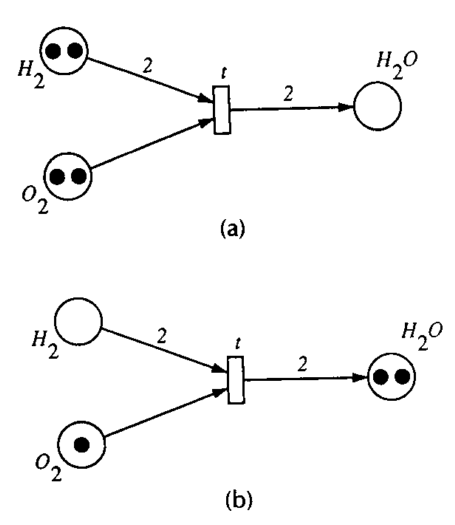
\includegraphics[width = 0.3\textwidth]	{resources/petri}
    	\legend{Regra de transição, (a) aceitação antes da transição \textbf{\textit{t}}. (b) iteração após aceitação de \textbf{\textit{t}}, \textbf{\textit{t}} está desativado.\cite{murata:1989}}
\end{figure}

\subsection{UML}
TODO.


\section{Visão Computacional}
Segundo \citeonline{marengoni:2009}, a visão computacional é uma forma de emular a visão humana, possuindo imagens como entrada, e sua saída é a interpretação dessa imagem.
Já \citeonline{bradski:2008}, definem uma parte da vasta área da visão computacional como uma transformação de dados de uma imagem em uma nova representação.

De acordo\citeonline{marengoni:2009}, o processamento da imagem geralmente é a primeira etapa do processo de visão computacional.
podendo ser dividido em três níveis: baixo-nível, nível-médio e alto-nível.
\begin{itemize}
\item Baixo-nível
	Pode ser associado a operações como redução de ruídos ou níveis de contraste da imagem.
\item Nível-médio
	São operações associadas a operações de segmentação de imagem ou reconhecimento de objetos na imagem.
\item Alto-nível
	São relacionados a tarefas de cognição associadas com a visão humana.
\end{itemize} 

\subsection{Pré-processamento de Imagem} \label{sect:preprocs}
\todo{melhorar esse texto 12/09/17}
Para evitar que imagens fiquem com interpretação limitada em determinados ambientes, por causa de diversos fatores como atenuação da luz e baixo contraste, é necessário pré-processá-las, para usar outros meios de processamento \cite{bazeille2006}. 

\subsection{Filtros para processamento digital de imagens}
TODO.

\subsubsection{Homomorphic filtering} 
	O filtro homomórfico (\textit{homomorphic filter}) é um filtro de frequência usado para corrigir iluminações não uniformes e realçar o contraste na imagem processada \cite{bazeille2006}.
     
 \begin{figure}[H]
	\centering
    	\caption{\label{fig:homofilter}Homomorphic Filtering}
		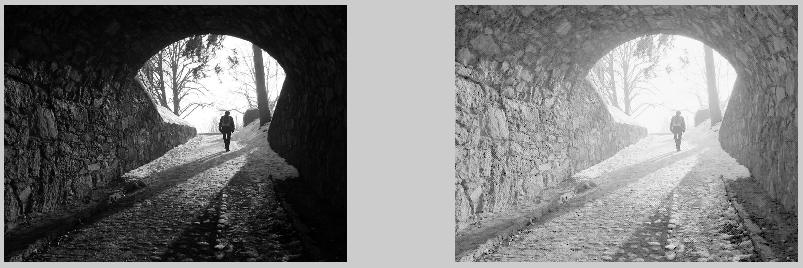
\includegraphics[width = 0.9\textwidth]	{resources/homofilter}
    	\legend{\textit{Homomorphic filtering}, usando \textit{Butterworth High Pass Filter} para fazer a filtragem \cite{mathworks:2008}}.
\end{figure}

    %Considerando o modelo de reflectância, assumimos que uma imagem é o produto descrito pela equação:
    \[
    %	f (x,y) = i(x,y).r(x,y)
    \]
    %Sendo $f(x,y)$ é a imagem captada por um sensor ótico, $i(x,y)$ o fator multiplicativo de iluminação e $r(x,y)$ a função de reflectância. 
    

\subsubsection{Anisotropic filtering}
O Filtro anisotrópico permite a simplificação de atributos da imagem para melhorar a segmentação,  suavizando as partes homogêneas preservando as bordas e melhorando-as.

 \begin{figure}[H]
	\centering
    	\caption{\label{fig:anisifilter}Anisotropic Filtering}
		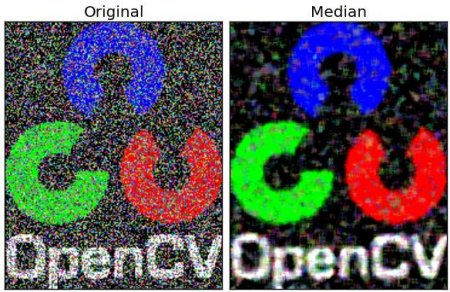
\includegraphics[width = 0.6\textwidth]	{resources/anisifilter}
    	\legend{Fonte:\cite{mathworks:2008}}.
\end{figure}

\subsection{Sensores de Aquisição de Imagens}
Segundo \citeonline{Lu:2017}, o som pode ser usado para mapear ambientes, emitindo um pulso que reflete no fundo do oceano criando um sonograma. As imagens obtidas por este sonar se assemelham a imagens óticas, com níveis de detalhes bem superiores. O reflexo criado por esse sonar tem formato de leque, com a medida que o pulso se movimenta, os reflexos irão criar séries de linhas de imagem, perpendiculares ao feixe.  

\subsection{Ferramentas para reconhecimento de images}
\todo{Definir junto ao método proposto}


\section{Reconhecimento de Padrões}

\todo{Definir junto ao método proposto}

\subsection{Aprendizado de máquina} 

\todo{Definir junto ao método proposto}

\subsection{Classificação de Padrões}




    


% ----------------------------------------------------------
% Revisão de Literatura
% ----------------------------------------------------------
\chapter{TRABALHOS CORRELATOS}
\label{chap:trab_cor}

\section{DeepFish: Accurate underwater live fish recognition with deep architecture}

\section{Automatic underwater image pre-processing}

\section{Foreground Extraction of underwater Videos via Sparse and Low-rank Matrix Decomposition}

\section{A Vision Based System for Object Detection in Underwater Images.}
\subsection{resumo}
O artigo propõe um sistema (véiculo autonomo) para detecção e rastreio de objetos submersos em água, o sistema faz detecção automática de canos (que podem se extender por kilometros). Utilizando procedimento para compensasão de cor foi desenvolvido para diminuir problemas causados pela luz, a identificação dos objetos é feita por uma rede neural, que classifica os pixels em tempo real, essa rede neural ajuda a navegação automática do veículo, traçando rotas e caminhos atráves das imagens processadas. Ressonância  geométrica é usada para diminuir a quantidade de detecções falsas, melhorar a precisão e mapear o ambiente, os sistemas de sonar foram desenvolvidos para melhorar a precisão da localização do veículo, não eliminando a utilização de um trasnponder.

\subsection{conclusão}
O sistema consegue detectar canos e outras estruturas, mesmo com os problemas causados pela falta de luminosidade, dispersão e atenuação da luz e outros problemas como areia sobre canos ou outros detritos; 


% ----------------------------------------------------------
% Detalhes de Desenvolvimento do Projeto
% ----------------------------------------------------------
\chapter{MÉTODO PROPOSTO}
\section{Big Picture}
    O sistema terá um sensor de captura ótica e sonora, que ficarão submersos em água, acoplados à uma boia, que terá um conexão sem fio com um celular ou computador.
\begin{figure}[h]
	\caption{\label{fig:bigpic}Visão Geral}
	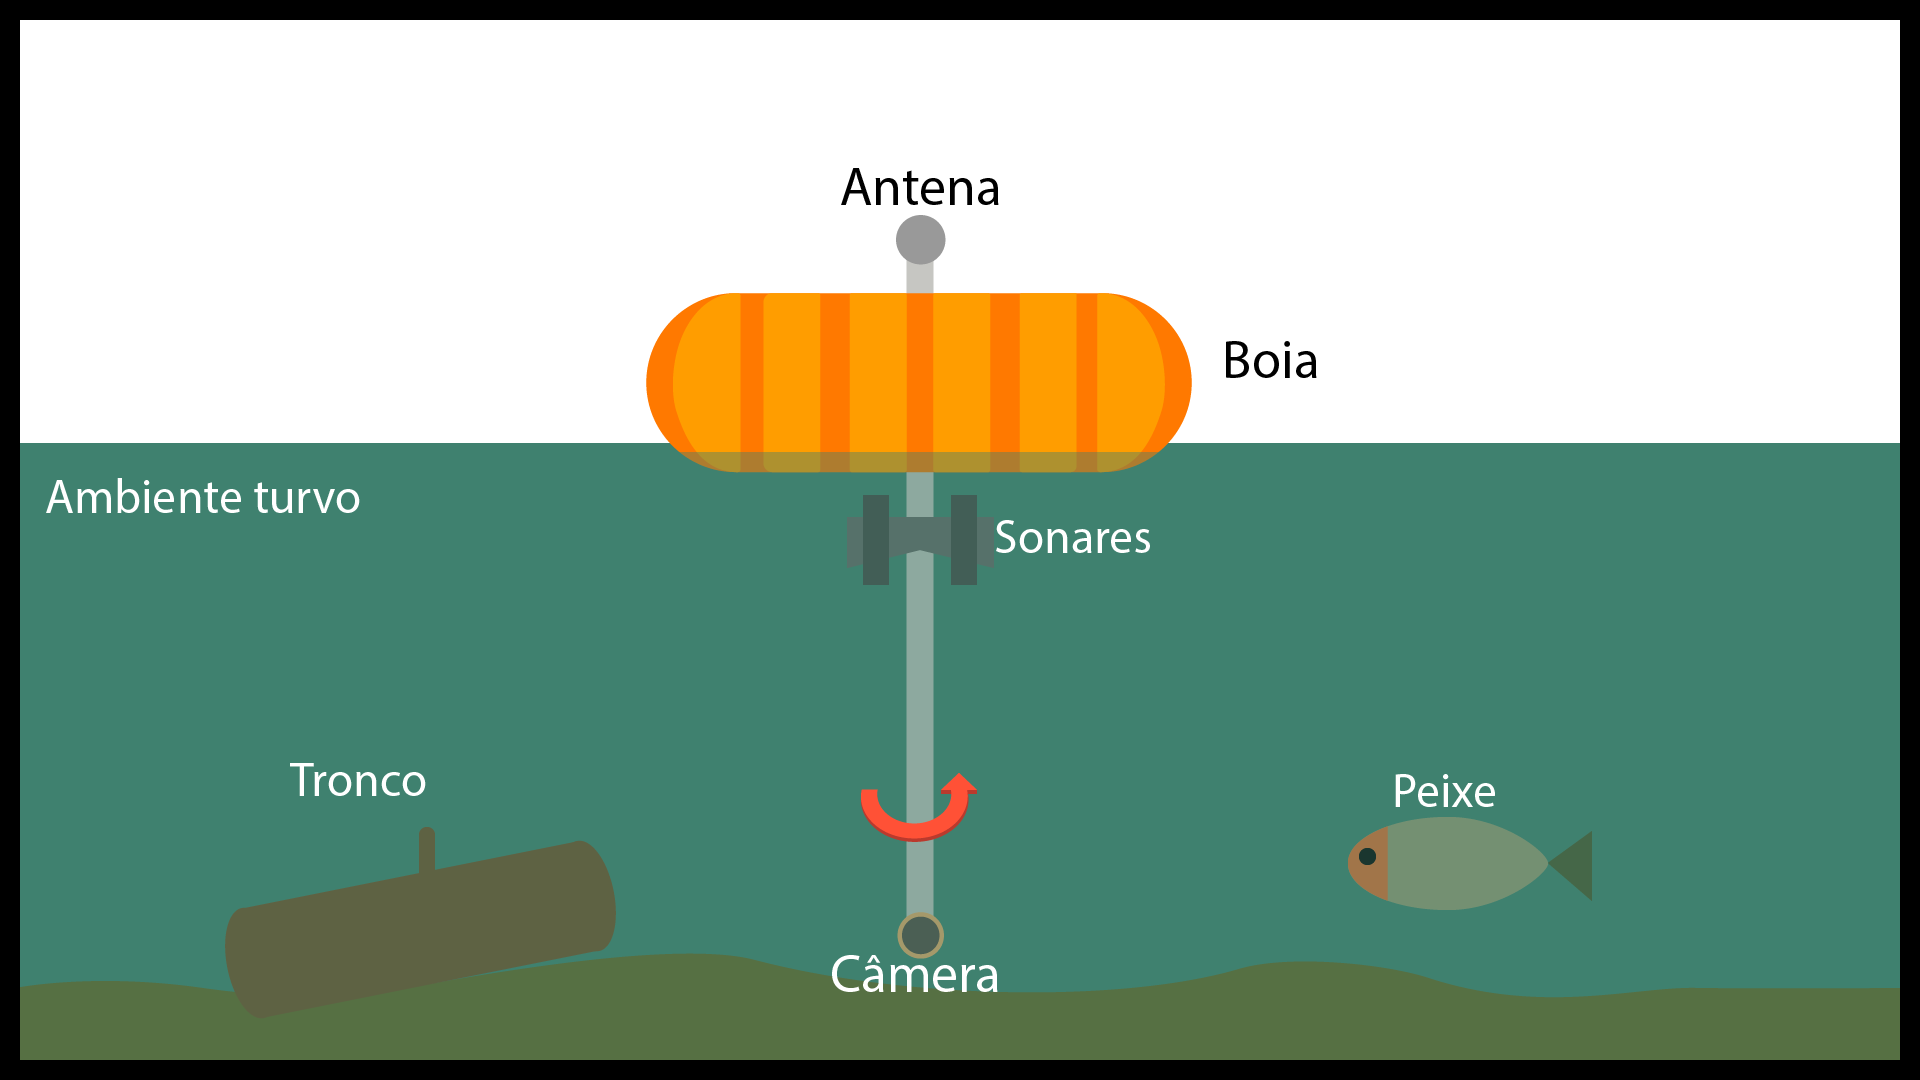
\includegraphics[width = 1\textwidth]			{resources/bigpicture}
    \legend{Fonte Própria}
\end{figure}

\todo{definir framework de processamento de imagens e algoritmos de classificação}

% ----------------------------------------------------------
% Cronograma
% ----------------------------------------------------------
\chapter{CRONOGRAMA}
\label{sec:cronograma}

A \autoref{fig:crono} exibe o cronograma proposto para a próxima etapa do trabalho de conclusão de curso, essas atividades são:

  \begin{description}  
  \item[Revisão da literatura sobre invariantes de memória:] Invariantes de memória adicionam condições de pré e pós execução de operações sobre memória, sendo importante para 
  este trabalho no que concerne a geração de \textit{witness}; 
  %
  \item[Aprimoramento do rastreamento de memória:] Comparar o rastreamento memória atual em outros modelos de memória, exemplo, o de precisão de \textit{bit} utilizado pelo VALGRING;
  %
  \item[Definição formal das propriedades de memória utilizado na verificação:] Criação de regras lógicas (baseada na lógica de inferência de Hoare \cite{Rocha:2015tese}) para as propriedades verificadas pelo Map2Check. 
  %
  \item[Aplicação de um \textit{slicer} de código para o Map2Check:] No modelo atual, a instrumentação do Klee pode gerar muitos casos e facilmente gerar um número excessivo de estados, assim como o Symbtiotic 3 \cite{Chalupa:2016} vamos utilizar um \textit{slicer} pra resolver esse problema.
  %
  \item[Adicionar \textit{bounded model checker} no método:] Com o uso de BMC será possível gerar outras propriedades de segurança de memória de forma mais otimizada, devido a aplicação de outras técnicas como \textit{Lazy Abstraction} \cite{Cordeiro:2012}
  %
  \item[Tradução das propriedades do \textit{bounded model checker}:] É necessário fazer com que o Map2Check seja compatível com a propriedades geradas pelo BMC, logo serão traduzidas as propriedades.
  %
  \item[Avaliação experimental das novas propriedades suportadas pelo método:] Testes empíricos sobre as novas funcionalidades.
  %
  \item[Realização de experimentos com \textit{benchmarks} públicos de programas escritos em C:] Com esses experimentos podemos verificar a eficácia real do método.
  %
  \item[Escrita de artigos:] Escrita de artigos para divulgação dos resultados do método.
  %
  \item[Finalização da monografia:] Escrita sobre tudo o que foi desenvolvido e estudado no trabalho.
  %
  \item[Apresentação final:] Defesa do trabalho de conclusão de curso.
\end{description}


\begin{table}[H]
	\caption{\label{fig:crono} Cronograma do projeto}
	\begin{center}
	    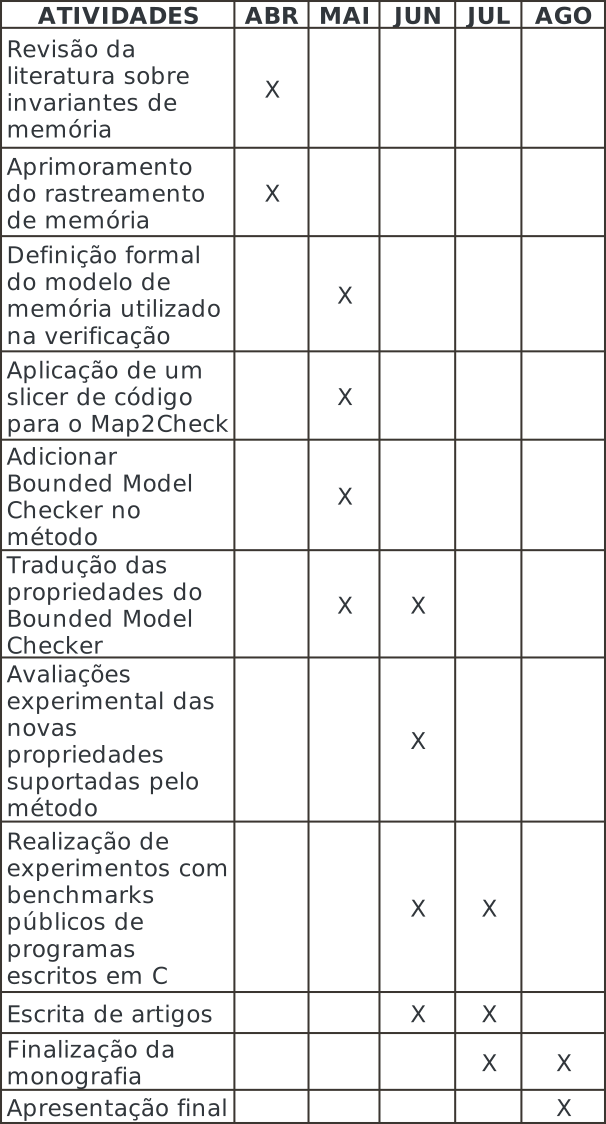
\includegraphics[scale=0.75]{resources/crono.png}
	\end{center}
	\legend{Fonte: Própria}
\end{table}

\newpage

% ----------------------------------------------------------
% Resultados -- Pode vir junto com discussão
% ----------------------------------------------------------
\chapter{RESULTADOS PARCIAIS}
%TODO: colocar especificações
% -----------------------------------------------------------------
% => RESULTADOS
% -----------------------------------------------------------------
\label{chapter:resultados}

Essa seção descreve o planejamento, projeto, execução e análise dos resultados de um estudo experimental para avaliar o método proposto neste trabalho quando aplicado 
em \textit{benchmark} públicos de programas em GNU-C ou ANSI-C. 

% -----------------------------------------------------------------
% => Planejamento e projeto dos experimentos
% -----------------------------------------------------------------
\section{Planejamento e projeto dos experimentos}
\label{sub:experimento}

Esta avaliação experimental visa avaliar a habilidade do Map2Check com LLVM em gerar e verificar casos de testes (assertivas) relacionados a gerência de memória, especificamente desalocações inválidas de memória. 
Neste sentido, foi definido as seguintes questões de pesquisa:
\begin{description}
\item[QP1:] Os casos de teste gerados pelo Map2Check são suficiente para identificação de uma desalocação inválida do programa analisado?
%
\item[QP2:] Qual a eficácia do Map2Check para detectar falhas de desalocações inválidas quando comparado com outras ferramentas?
%
\item[QP3:] O método proposto aprimora a detecção de falhas de desalocações inválidas quando comparado a versão anterior do Map2Check?
\end{description}

Visando responder essas questões, foram utilizados $14$ programas da categoria 
\textit{MemorySafety} do \textit{benchmark} da \textit{Competition on Software Verification} (SV-COMP) \cite{beyer:2016}. Estes programas são classificados com \texttt{FALSE(valid-free)}, ou seja, esses programas contém desalocação inválida de memória. O SV-COMP é uma competição internacional onde diversas ferramentas são submetidas a \textit{benchmark} públicos (obtidos de diferentes domínios como \textit{drivers} e \textit{kernel} do Linux) e depois avaliadas e pontuadas. Assim, o SV-COMP tem como objetivo avaliar a transferência de tecnologia e comparar verificadores de software no estado da arte em relação à eficácia e eficiência. 
%Na categoria \textit{MemorySafety} foram pegos os 

\par
Nos \textit{benchmarks} da SV-COMP, alguns programas adotam funções específicas, por exemplo, a categoria de \textit{MemorySafety} contém a função \texttt{\_\_VERIFIER\_nondet\_int} que modela valores não determinísticos de inteiros. No Map2Check, foi implementado uma instrumentação para que o Klee (utilizando execução simbólica) gere os valores necessários para explorar os caminhos de execução do programa e então efetuar a verificação das assertiva nos  programas analisados.

\par
A execução da ferramenta Map2Check para avaliar os \textit{benchmarks} foi feita utilizando a ferramenta Benchexec \cite{beyer:2015} que gerencia, monitora e faz medidas de recursos (memória e tempo de execução pela CPU) utilizados por ferramentas. 
%
No Benchexec foram adotas as seguintes configurações para execução do experimento: 
um tempo máximo de execução (\textit{timeout}) de 15 minutos por programa a ser analisado, ou seja, se o Map2Check não chegar a uma conclusão dentro desse tempo, a execução será interrompida; 
%para aquela entrada e a próxima será executada (e o resultado do teste será uma indeterminação). 
$8$ GB de memória RAM; e 
$5$ núcleos de processador.  
A máquina utilizada para execução do experimento continha um sistemas operacional Linux Ubuntu $16.10$ com $16$GB de memória, processador AMD $2.9$ GHz com $8$ cores de CPU. 
%
%Antes da execução já se sabia que no momento atual a implementação atual do Map2Check não %suporta \textit{loops} e o Klee pode gerar muitos valores simbólicos causando ocupação de um %espaço muito grande de memória. Então o foco da análise foi em verificar a quantidade de %falsos positivos e de falsos negativos que a ferramenta geraria.

\par
A avaliação foi conduzida da seguinte forma: 
(1) Aplicação do Map2Check sobre os programas do \textit{benchmark} do SV-COMP; 
(2) Comparação dos resultados obtidos (diretamento da página oficial do SV-COMP) com a versão anterior do Map2Check\footnote{https://sv-comp.sosy-lab.org/2016/results/results-verified/META\_Heap.table.html} \cite{beyer:2016}, ESBMC e Symbiotic 4\footnote{https://sv-comp.sosy-lab.org/2017/results/results-verified/META\_MemSafety.table.html}. 
Vale ressaltar que nos resultados da versão anterior do Map2Check no SV-COMP de 2016 havia um programa a menos na categoria \textit{MemorySafety}.

% -----------------------------------------------------------------
% => Execução dos experimento e Análise dos Resultados
% -----------------------------------------------------------------
\section{Execução dos experimento e Análise dos Resultados}

Após a execução dos \textit{benchmarks}, foram obtidos os resultados mostrados na \autoref{tabela:resultados}, onde cada linha da tabela contém: 
(1) nome da ferramenta (Ferramenta); 
(2) número de programas que a ferramenta identificou corretamente (Corretos); 
(3) número de programas que a ferramenta identificou um erro para um programa que atende todas as especificações (Falsos Negativo); 
(4) número de programas em que a ferramenta falhou para computar a verificação (Desconhecidos); e 
(5) número de programas avaliados (Total).

\begin{table}[H]
	\caption{\label{tabela:resultados} Resultado da experimentação}
	\begin{center}
	    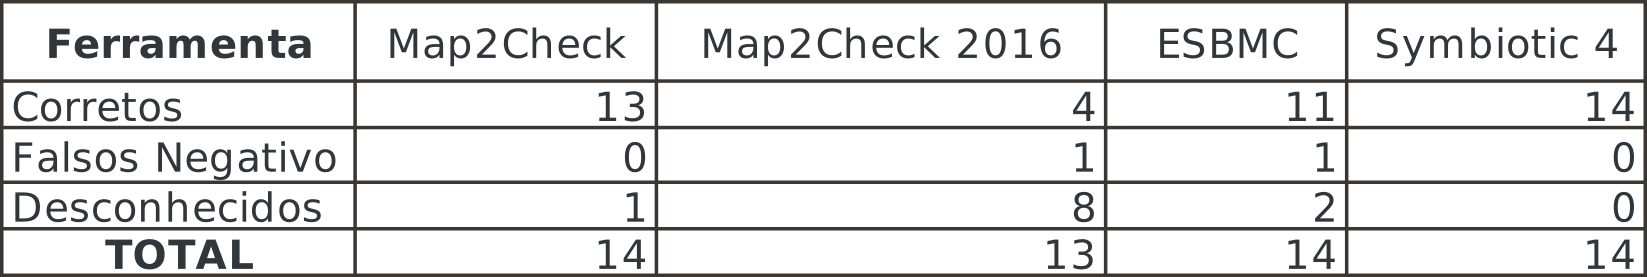
\includegraphics[scale=0.33]{resources/tabelaResultados.png}
	\end{center}
	\legend{Fonte: Própria}
\end{table}

Para respondermos a questão de pesquisa \textbf{QP1} e \textbf{QP2} da \autoref{sub:experimento}, foi analisado a \autoref{tabela:resultados} que mostra que o Map2Check classificou corretamente aproximadamente $93\%$ dos programas avaliados, enquanto o Simbiotic $4$  classificou corretamente  $100$\%, o ESBMC classificou corretamente  aproximadamente $79$\%. O Map2Check não gerou nenhum falso positivo nem falso negativo, foi gerado apenas um resultado desconhecido, acredita-se que é um caso de melhorias para a execução simbólica, por exemplo, por meio da aplicação de um \textit{slicer} de código \cite{Chalupa:2016}. 
%foi pela não utilização de um \textit{model checker}. %
No futuro, é planejado adotar um \textit{slicer}, bem como, um \textit{model checker} para ampliar o conjunto de propriedades inferidas, como é apresentado na \autoref{sec:cronograma}. 

\par
Com respeito  a questão de pesquisa \textbf{QP3} da \autoref{sub:experimento}, utilizando \autoref{tabela:resultados} podemos comparar os resultados, visando uma comparação mais justa, foi excluído o programa que a versão anterior do Map2Check não analisou e como a versão atual categorizou esse programa de forma correta, vamos subtrair 1 do total de corretos. A nova versão do Map2Check então classificou corretamente 92\% dos casos e a versão antiga 31\%. A versão antiga havia gerado um falso negativo enquanto a nova não gerou nenhum.
%\par
Os resultados, embora preliminares em natureza, sugerem fortemente que o método pode ser eficaz em gerar e validar casos de teste para verificação de desalocações inválidas de programas em C. Vale ressaltar que novos experimentos serão realizados a fim de determinar a eficácia da nova versão do Map2Check com LLVM.

%Então, pode-se defender de que o Map2Check integra teste e verificação. O teste é baseado é %análise dinâmica e verificação de assertivas. As assertivas contém um conjunto de %especificações.
%\chapter{DISCUSSÃO}

% ----------------------------------------------------------
% Conclusão
% ----------------------------------------------------------
\chapter{CONSIDERAÇÕES PARCIAIS E PRÓXIMOS PASSOS}
\label{chapter:consideracoes}

Neste trabalho foi apresentado a importância da verificação de \textit{software} para validar propriedades de segurança no gerenciamento de memória. Foi descrito um método proposto para aprimorar o método Map2Check além da implementação do mesmo, que é capaz de gerar, verificar e validar propriedades de segurança no gerenciamento de memória em programas em C. Adicionalmente, foi apresentado um avaliação experimental comparado a eficácia da ferramenta em relação a outras ferramentas com propostas similares. 
\par
O método até o presente momento é capaz de gerar, verificar e validar propriedades de segurança para desalocações inválidas, não gera o \textit{witness} no formato descrito em \citeonline{beyer:2016}, mas apresenta um log de rastreamento  
%(para o \textit{witness} utilizar)
com dados sobre a violação das propriedades. 
 novo método quando comparado a versão anterior no quesito desalocações inválidas, o novo método apresentou melhorias significativas quanto a eficácia (segundo o \textit{benchmark} da SV-COMP'17), quando comparado as ferramentas atuais (SYMBIOTIC 4 \cite{Chalupa:2016} e ESBMC \cite{Cordeiro:2012} ), foi verificado que o Map2Check foi mais eficaz que o ESBMC e por apenas um programa, menos eficaz que SYMBIOTIC 4, que segundo \citeonline{beyer:2016} são ferramentas que usualmente apresentam bons resultados (obtendo posições no \textit{ranking}) no SV-COMP. Além disso, o Map2Check não gerou nenhum falso positivo, o que sugere que o método proposto é eficaz mesmo quando comparado a outras ferramentas.  
 
 \par
%\todo{corrigir formatação deste paragrafo}
Na próxima etapa deste trabalho serão adicionadas novas funcionalidades ao método, entre elas: geração de \textit{witness} no formato descrito em \citeonline{beyer:2016} utilização de um \textit{model checker} para inferência de novas propriedades adoção de um \textit{slicer} de código; e 
validação de vazamentos de memória. 
Desta forma, espera-se que o Map2Check seja capaz de verificar e validar programas em C com mais eficiência e eficácia e assim solucionar o problema proposto por esse trabalho.  
%\todo{Nas referências remover os textos com Citado X vezes por...; Nas referências manter padrão hora em maisculo ou minúscula}. 
\newpage
% ----------------------------------------------------------
% Referências bibliográficas
% ----------------------------------------------------------
\bibliography{main}

%---------------------------------------------------------------------
% INDICE REMISSIVO
%---------------------------------------------------------------------
%\phantompart
\printindex
%---------------------------------------------------------------------

\end{document}
